\documentclass[a4paper,12pt]{article}
\usepackage[utf8]{inputenc}
\setlength{\marginparwidth}{2cm}
\usepackage{todonotes}
\usepackage[russian]{babel}
\usepackage{graphicx}
\usepackage{amsmath, amssymb}
\usepackage{hyperref}
\usepackage{float}
\usepackage{listings}
\usepackage{caption}
\usepackage{geometry}
\usepackage{xcolor}
\geometry{left=2cm,right=2cm,top=2cm,bottom=2cm}
\hypersetup{pdfborder=0 0 0}
\headsep=8mm
\footskip=20mm
\hypersetup{pdfstartview=FitH, linkcolor=linkcolor, urlcolor=urlcolor, colorlinks=true}

\definecolor{strings}{rgb}{0,0.6,0}
\definecolor{comments}{rgb}{0,0.3,0}
\definecolor{numbers}{rgb}{0.5,0.5,0.5}
\definecolor{keywords}{rgb}{0.09,0.61,0.95}
\definecolor{background}{rgb}{0.97,0.97,0.97}

\lstdefinestyle{codestyle}{
    backgroundcolor=\color{background},
    commentstyle=\color{comments},
    keywordstyle=\color{keywords},
    stringstyle=\color{strings},
    numberstyle=\tiny\color{numbers},
    basicstyle=\ttfamily\scriptsize,
    breakatwhitespace=false,
    breaklines=true,
    captionpos=b,
    inputencoding=utf8,
    keepspaces=false,
    numbers=left,
    numbersep=5pt,
    showspaces=false,
    showstringspaces=false,
    showtabs=false,
    tabsize=2,
    extendedchars=true
}

\lstset{style=codestyle}

\begin{document}    

% Титульный лист
\begin{titlepage}
    \centering
    {\large Федеральное государственное автономное образовательное учреждение\par}
    {\large высшего образования\par}
    {\bfseries САНКТ-ПЕТЕРБУРГСКИЙ НАЦИОНАЛЬНЫЙ ИССЛЕДОВАТЕЛЬСКИЙ УНИВЕРСИТЕТ ИТМО\par}
    {\bfseries Факультет систем управления и робототехники\par}
    \vfill
    {\Large \bfseries Лабораторная работа №1\par}
    {\Large \bfseries Градиентный спуск \par}
    \vfill
    
    \begin{flushright}
        Студенты: Бахтаиров Р.А.,\\ Сайфуллин Д.Р. \\
        Группа:  R3243\\
        Преподаватель: Попов А.М.
    \end{flushright}
    \vfill
    Санкт-Петербург,\\ 
    2025 г.
\end{titlepage}

\section{Введение}
В данной лабораторной работе реализованы и исследованы методы оптимизации: методы нулевого порядка (золотое сечение, параболы, Брент), градиентный спуск с различными стратегиями выбора шага, а также построение траектории с использованием потенциальной функции. Все методы протестированы на заданных функциях, включая мультимодальные, с построением графиков сходимости и анализом результатов. \\[0.5em]
\textit{Примечание: весь код для выполнения работы находится в файле \texttt{main.ipynb}.}
\section{Одномерная оптимизация нулевого порядка}

\subsection{Реализация методов}
Реализованы следующие методы:
\begin{itemize}
    \item \textbf{Метод золотого сечения}: сужение интервала с использованием $\phi = \frac{1 + \sqrt{5}}{2}$.
    \item \textbf{Метод парабол (явная формула)}:
    \[
    u = x_2 - \frac{(x_2 - x_1)^2 (f(x_2) - f(x_3)) - (x_2 - x_3)^2 (f(x_2) - f(x_1))}{2 \left( (x_2 - x_1) (f(x_2) - f(x_3)) - (x_2 - x_3) (f(x_2) - f(x_1)) \right)}
    \]
    \item \textbf{Метод парабол (солвер)}: аппроксимация параболы через три точки с решением системы уравнений $ax^2 + bx + c = f(x)$.
\end{itemize}

\subsection{Тестовые функции}
В первом задании необходимо протестировать реализованные методы на следующих функциях:
\begin{enumerate}
    \item $f(x) = -5x^5 + 4x^4 - 12x^3 + 11x^2 - 2x + 1$ на $[-0.5, 0.5]$
    \item $f(x) = -\ln^2(x-2) + \ln^2(10-x) - x^{0.2}$ на $[6, 9.9]$
    \item $f(x) = -3x \sin(0.75x) + e^{-2x}$ на $[0, 2\pi]$
    \item $f(x) = e^{3x} + 5e^{-2x}$ на $[0, 1]$
    \item $f(x) = 0.2x \ln x + (x-2.3)^2$ на $[0.5, 2.5]$
\end{enumerate}

\subsection{Анализ}
Построим графики сходимости методов для каждой из функций и сравним результаты.
\begin{figure}[H]
    \begin{minipage}{0.49\textwidth}
                \centering 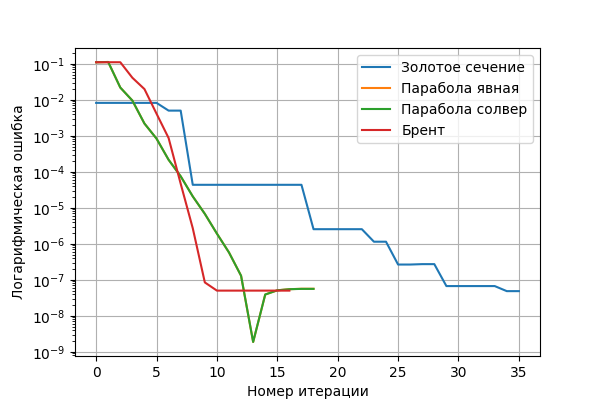
\includegraphics[width=\textwidth]{images/task1/f1.png}
        \caption{Сходимость методов для функции 1}
    \end{minipage}\hfill
    \begin{minipage}{0.49\textwidth}
        \centering 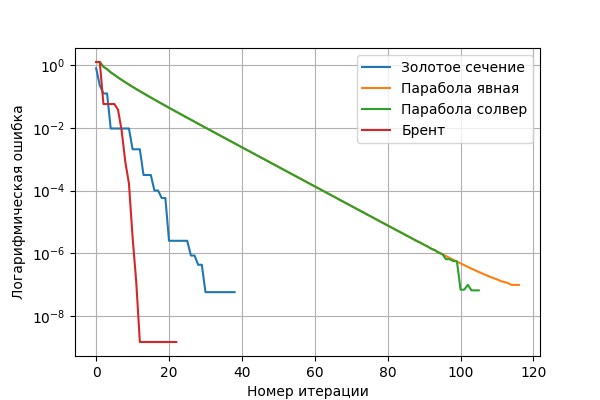
\includegraphics[width=\textwidth]{images/task1/f2.png}
        \caption{Сходимость методов для функции 2}
    \end{minipage}
\end{figure}
\begin{figure}[H]
    \begin{minipage}{0.49\textwidth}
        \centering 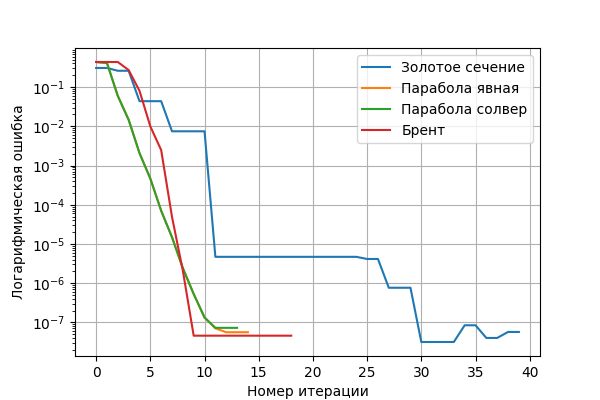
\includegraphics[width=\textwidth]{images/task1/f3.png}
        \caption{Сходимость методов для функции 3}
    \end{minipage}\hfill
    \begin{minipage}{0.49\textwidth}
        \centering 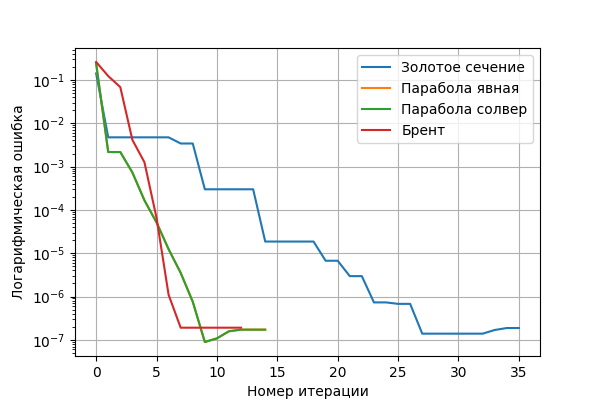
\includegraphics[width=\textwidth]{images/task1/f4.png}
        \caption{Сходимость методов для функции 4}
    \end{minipage}
\end{figure}
\begin{figure}[H]
    \centering
    \begin{minipage}{0.49\textwidth}
        \centering 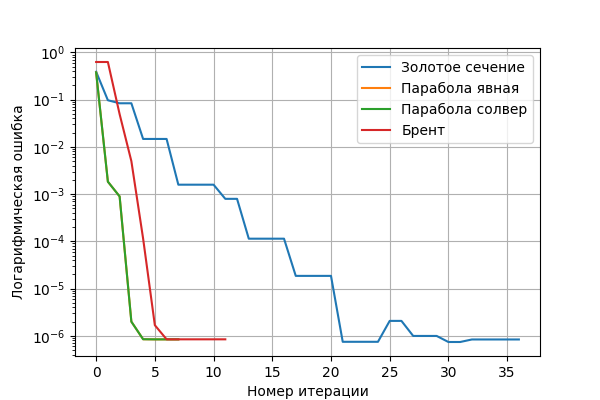
\includegraphics[width=\textwidth]{images/task1/f5.png}
        \caption{Сходимость методов для функции 5}
    \end{minipage}
\end{figure}
Анализируем результаты:
\begin{enumerate}
    \item На графике видно, что метод золотого сечения сходится медленнее всех: ошибка убывает ступенчато и лишь к 15--20 итерации достигает порядка $10^{-7}$. Методы парабол (как явная формула, так и через solve) и Брента выходят на точность $10^{-7}\!-\!10^{-8}$ гораздо быстрее (примерно к 7--10 итерации). В итоге наименьшее число итераций показывает метод Брента.
    \item Здесь параболический метод через solve (зелёная кривая) убывает по логарифмической шкале почти линейно, то есть довольно медленно достигает нужной точности (лишь к 100+ итерациям ошибка около $10^{-8}$). Зато метод Брента (красная кривая) очень быстро (к 15--20 итерации) падает до $10^{-8}$. Золотое сечение (синяя кривая) тоже быстрее, чем «парабола solve», но чуть отстаёт от Брента. Парабола (явная формула) (оранжевая кривая) в итоге добирается к точности $10^{-8}$ чуть раньше 110 итераций.
    \item Методы парабол (зелёная и оранжевая) и Брента (красная) снова сходятся заметно быстрее золотого сечения. При этом Брент и «парабола solve» достигают порядка $10^{-7}$ уже на 5--7 итерации, тогда как золотое сечение выходит на ту же точность ближе к 15 итерации. Разница между параболическими методами здесь не столь велика: оба быстро уменьшают ошибку.
    \item Аналогично, золотое сечение идёт «ступеньками» и лишь к 25--30 итерации выходит на $10^{-7}$. Параболические методы и Брент делают это существенно быстрее (уже около 7--10 итерации). При этом метод Брента чуть обгоняет «параболу solve», а явная парабола примерно посередине.
    \item На данном графике видно, что уже к 5--7 итерации методы Брента (красная) и парабол (зелёная) достигают уровня $10^{-7}$, в то время как золотое сечение (синяя кривая) лишь к 15--20 итерации подходит к той же точности. Парабола (явная формула) (оранжевая) ведёт себя близко к «параболе solve», но иногда чуть медленнее на начальных шагах.
\end{enumerate}
По приведённым графикам можно сделать следующие наблюдения:
\begin{itemize}
    \item Методы, использующие параболическую интерполяцию (парабола и Брент), как правило, сходятся быстрее, чем «чистое» золотое сечение.
    \item Метод Брента почти во всех примерах демонстрирует наивысшую скорость сходимости, достигая заданной точности за наименьшее число итераций.
    \item «Парабола solve» иногда даёт чуть медленнее сходимость, если при построении системы уравнений возникают неблагоприятные численные условия, но всё равно обгоняет золотое сечение.
    \item «Парабола заданная явной формулой» обычно ведёт себя похоже на «параболу solve», иногда сходится быстрее, иногда медленнее --- это зависит от свойств целевой функции и точности вычислений.
\end{itemize}

Теперь попробуем использовать встроенный оптимизатор \texttt{scipy.optimize.minimize} для каждого метода и сравним с результатом работы нашего алгоритма. Построим графики:
\begin{figure}[H]
    \begin{minipage}{0.49\textwidth}
                \centering 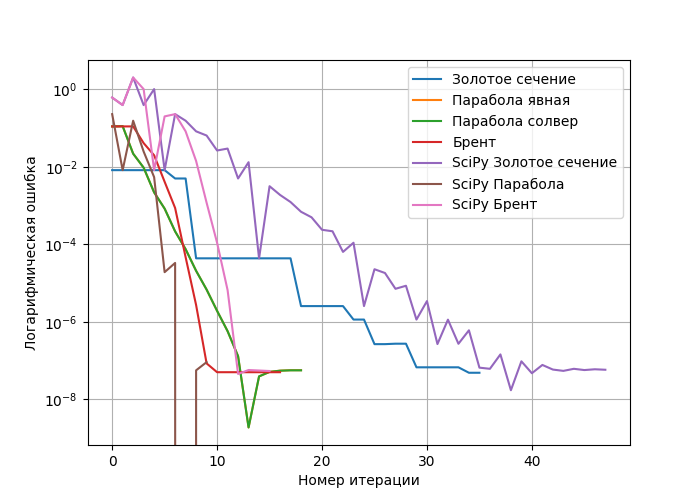
\includegraphics[width=\textwidth]{images/task1/f1_with_scipy.png}
        \caption{Сходимость методов для функции 1}
    \end{minipage}\hfill
    \begin{minipage}{0.49\textwidth}
        \centering 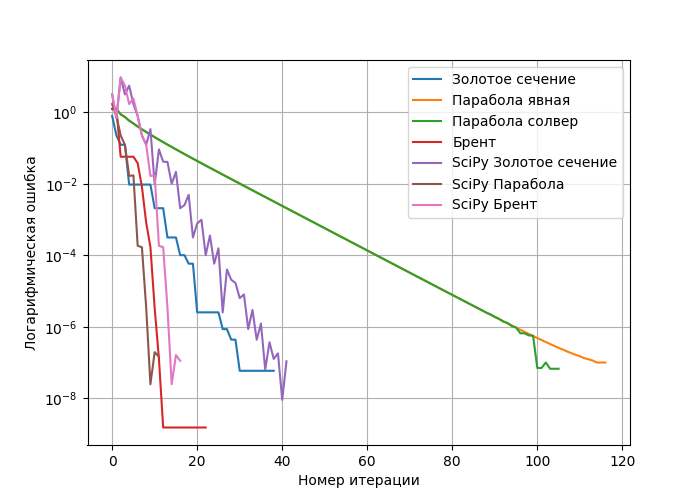
\includegraphics[width=\textwidth]{images/task1/f2_with_scipy.png}
        \caption{Сходимость методов для функции 2}
    \end{minipage}
\end{figure}
\begin{figure}[H]
    \begin{minipage}{0.49\textwidth}
        \centering 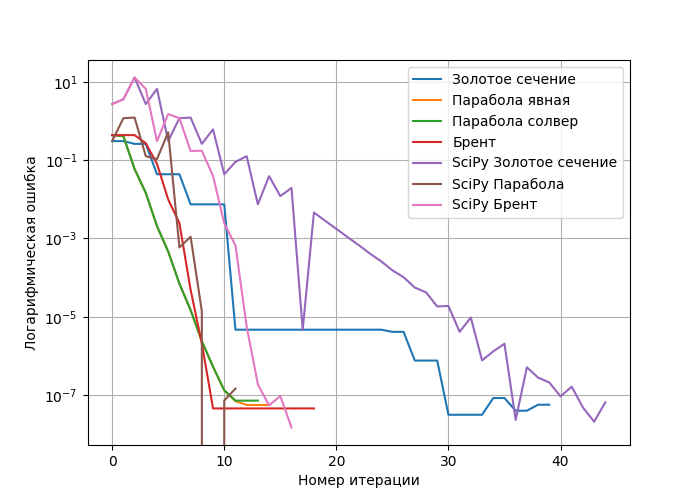
\includegraphics[width=\textwidth]{images/task1/f3_with_scipy.png}
        \caption{Сходимость методов для функции 3}
    \end{minipage}\hfill
    \begin{minipage}{0.49\textwidth}
        \centering 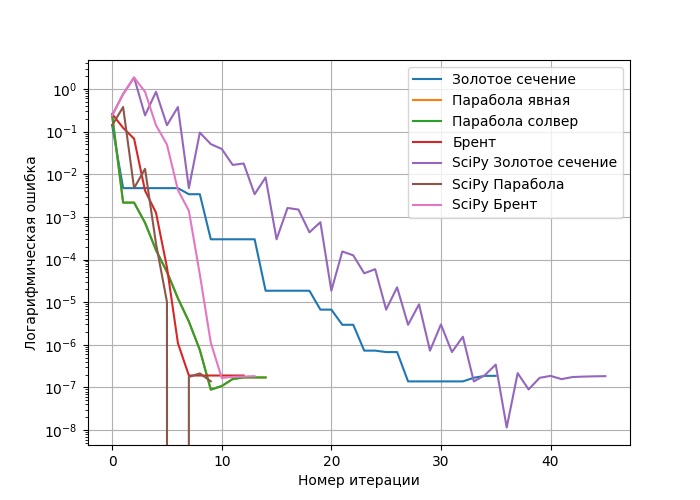
\includegraphics[width=\textwidth]{images/task1/f4_with_scipy.png}
        \caption{Сходимость методов для функции 4}
    \end{minipage}
\end{figure}
\begin{figure}[H]
    \centering
    \begin{minipage}{0.49\textwidth}
        \centering 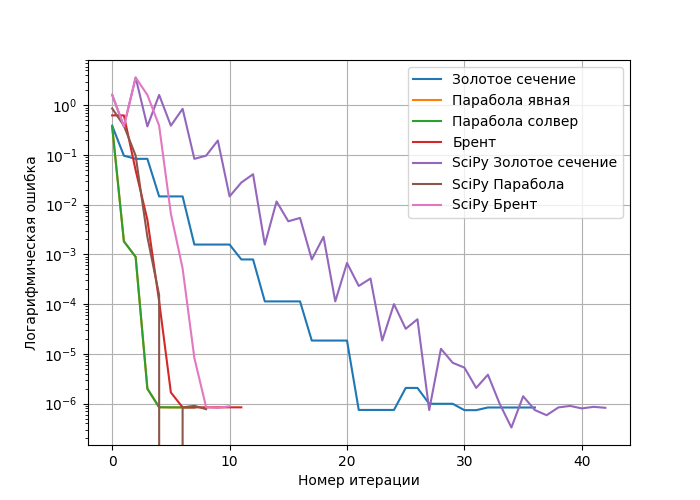
\includegraphics[width=\textwidth]{images/task1/f5_with_scipy.png}
        \caption{Сходимость методов для функции 5}
    \end{minipage}
\end{figure}
По приведённым графикам можно сделать следующие наблюдения:
\begin{enumerate}
    \item На графике видно, что методы Брента (красная) и парабол (зелёная и оранжевая) достигают уровня $10^{-7}$ существенно быстрее золотого сечения (синяя кривая). При этом «SciPy Брент» и «SciPy Парабола» тоже показывают быструю сходимость, в то время как «SciPy Золотое сечение» идёт более ступенчато.
    \item Параболический метод через solve (зелёная кривая) здесь убывает почти линейно в логарифмическом масштабе и достигает точности порядка $10^{-8}$ только ближе к 100-й итерации. Зато метод Брента (наш и из SciPy) выходит на ту же точность гораздо раньше (примерно к 15--20 итерации). Золотое сечение (наше и SciPy) идёт быстрее «параболы solve», но отстаёт от Брента.
    \item Методы парабол (оранжевая и зелёная) и Брента (красная) снова сходятся заметно быстрее золотого сечения (синяя). При этом «SciPy Брент» (розовая) и «SciPy Парабола» (чёрная) также показывают быстрый спад ошибки, в отличие от «SciPy Золотого сечения» (фиолетовая), которое идёт более плавно и достигает $10^{-7}$ позже.
    \item Аналогично, золотое сечение идёт «ступеньками» и лишь к 25--30 итерации достигает ошибки порядка $10^{-7}$. Параболические методы (оба варианта) и Брент делают это гораздо быстрее, уже к 10--12 итерации. SciPy-реализации ведут себя сходным образом: «SciPy Брент» и «SciPy Парабола» выходят на малую ошибку быстрее, чем «SciPy Золотое сечение».
    \item На данном графике видно, что уже к 5--7 итерации методы Брента (красная и розовая) и парабол (зелёная, оранжевая, чёрная) выходят на уровень $10^{-7}$, тогда как золотое сечение (синяя и фиолетовая) лишь к 15--20 итерации. При этом «Парабола solve» иногда чуть запаздывает, если система уравнений даёт неблагоприятные числа, но всё равно опережает золотое сечение.
\end{enumerate}

В пятом пункте требуется рассмотреть 2 мультимодальные функции, построить их графики и найти точки минимума каждым из методов. Будем исследовать следующие функции:
\begin{enumerate}
    \item $f_1(x) = (x^2 - 3)^2 + \sin(5x)$ на отрезке $[-2, 3]$. Данная функция сочетает квадратичный компонент $(x^2 - 3)^2$, имеющий минимум при $x = \pm\sqrt{3}$, и колебательную часть $\sin(5x)$, которая добавляет несколько локальных минимумов.
    \item $f_2(x) = 0.1\,x^2 + \cos(3x) + 2\sin(5x)$ на отрезке $[-2, 2]$. Здесь квадратичный член $0.1\,x^2$ даёт «параболическое» возрастание на больших $|x|$, а сумма $\cos(3x) + 2\sin(5x)$ порождает множественные «волны» и локальные впадины.
\end{enumerate}

Для каждой из этих функций запустим реализованные методы: золотое сечение, парабола (явная формула), парабола (через solve) и Брент. На рисунках ниже показаны графики каждой функции и отмечены точки, куда сошёлся тот или иной метод, а также приведена логарифмическая ошибка на каждом шаге (при наличии логов итераций).

\begin{figure}[H]
    \centering
    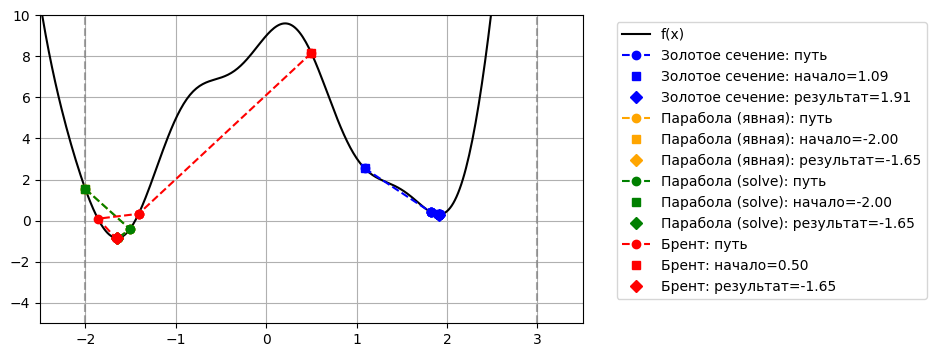
\includegraphics[width=\textwidth]{images/task1/multifunc_1.png}
    \caption{График функции $f_1(x)$ и результаты методов на отрезке $[-2,3]$.}
\end{figure}

\begin{figure}[H]
    \centering
    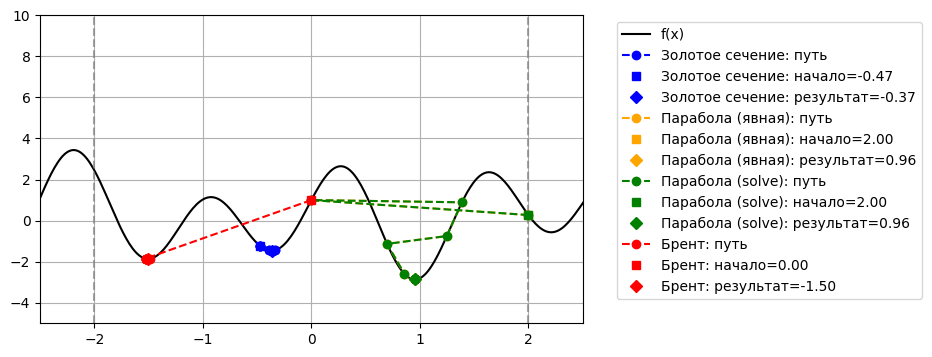
\includegraphics[width=\textwidth]{images/task1/multifunc_2.png}
    \caption{График функции $f_2(x)$ и результаты методов на отрезке $[-2,2]$.}
\end{figure}
Анализируем графики и делаем следующие выводы:
\begin{enumerate}
    \item На первом графике видно, что при начальных приближениях в диапазоне от $x=-2.0$ до $x=0.5$ методы «Парабола» (явная и solve) и Брент смещаются в локальный минимум около $x\approx -1.65$, тогда как «Золотое сечение» при старте с $x\approx1.09$ уходит к другому локальному минимуму вблизи $x\approx1.91$. Это показывает, что разные начальные условия (или интервалы) приводят к поиску разных локальных впадин при мультимодальной форме $f(x)$.
    \item На втором графике функции, имеющей несколько волн на отрезке $[-2,2]$, видно, что метод Брента (красная кривая), начав с $x=0.00$, уходит к минимуму около $x=-1.50$, «Золотое сечение» (синий) при старте с $x\approx-0.47$ попадает в точку $x\approx-0.37$, а «Парабола» (явная и solve) при $x=2.00$ сходится к минимуму около $x=0.96$. Таким образом, каждая пара «старт + метод» нашла свою локальную впадину, что ещё раз подчёркивает, что унимодальные алгоритмы без многократного запуска не гарантируют нахождение глобального минимума при наличии нескольких локальных.
\end{enumerate}

\subsection{Выводы}
\begin{enumerate}
    \item На тестовых унимодальных функциях все методы успешно сходятся к точке минимума, однако методы с параболической аппроксимацией и метод Брента достигают заданной точности быстрее, чем золотое сечение; это подтверждается графиками логарифмической ошибки: золотое сечение даёт более ступенчатое уменьшение, а параболы и Брент часто выходят на значения $10^{-7}$--$10^{-8}$ за меньшее число итераций.
    \item При сравнении с методами SciPy наблюдается схожая тенденция: реализация golden в \texttt{minimize\_scalar} работает похожим образом на наше золотое сечение, а brent и bounded сходятся существенно быстрее; разница в точном числе итераций объясняется внутренними эвристиками SciPy и разными критериями остановки, однако общее преимущество параболических методов и Брента остаётся.
    \item При тестировании на мультимодальных функциях все унимодальные алгоритмы (золотое сечение, парабола, Брент) могут находить разные локальные минимумы в зависимости от начального приближения или заданного отрезка, то есть ни один из рассмотренных методов не гарантирует поиск глобального минимума, если функция имеет несколько впадин на заданном интервале; это подтверждают графики, где каждый метод останавливается в своей локальной точке.
    \item Таким образом, для унимодальных задач методы парабол и Брента обеспечивают более быструю сходимость по сравнению с золотым сечением, а для мультимодальных функций без дополнительных приёмов (например, многократных запусков или глобальных алгоритмов) нет гарантии найти глобальный минимум.
\end{enumerate}

\section{Градиентный спуск}
По заданию требуется реализовать следующие стратегии:
\begin{itemize}
    \item Постоянный шаг: $\alpha_k = \text{const}$.
    \item Поиск $\beta$: минимизация вдоль направления с использованием методов нулевого порядка, $\alpha_k = \frac{\beta}{\|\nabla f(x_k)\|}$.
    \item Адаптивный шаг: $\alpha_k = \frac{1}{L_k}$ (константа Липшица).
    \item Армихо-Вульф: backtracking для выбора шага.
\end{itemize}
Для визуализации результатов работы стратегий рассмотрим задачу минимизации квадратичной функции
$f(x) \;=\; x^\mathsf{T} A x \;+\; b^\mathsf{T} x,$
где $A = \begin{bmatrix} 2 & 1 \\ 1 & 2 \end{bmatrix}$, $b = \begin{bmatrix} -1 \\ 1 \end{bmatrix}$. \\[0.5em]
Аналитически решение задаётся $\nabla f(x^*)=0$, то есть $2A\,x^* + b=0$, откуда $x^* = -\tfrac12\,A^{-1} b$. Константа Липшица: $L = 2\lambda_{\max}(A)$.\\[0.5em]
Мы запускаем градиентный спуск с четырьмя стратегиями выбора шага и сравниваем их поведение на нескольких начальных приближениях.
\subsection{Анализ}
Протестируем алгоритм с каждой их стратегий, построим 2D- 3D-графики и отметим на них результат работы траекторий. 
\begin{figure}[H]
    \begin{minipage}{0.49\textwidth}
        \centering 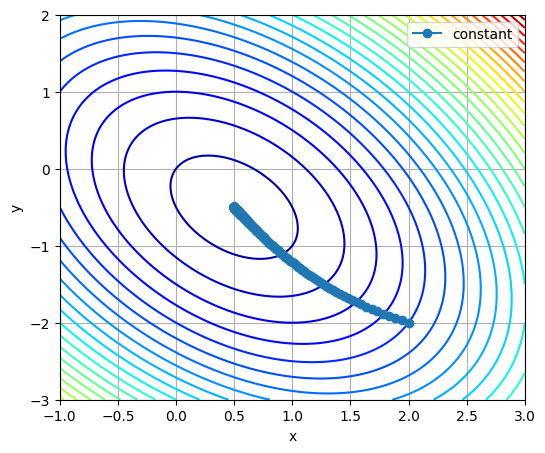
\includegraphics[width=\textwidth]{images/task2/plot_levels_2_2_constant.png} 
        \caption{Линии уровня, constant.}
    \end{minipage}\hfill
    \begin{minipage}{0.49\textwidth}
        \centering 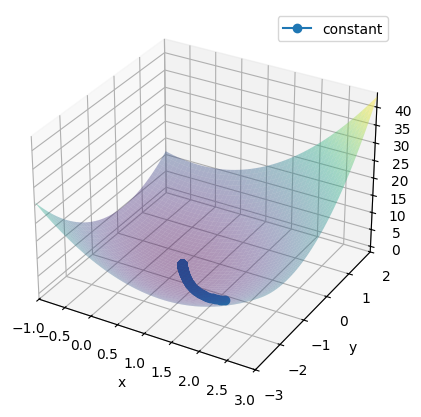
\includegraphics[width=0.84\textwidth]{images/task2/plot_3d_2_2_constant.png}
        \caption{3D-график, constant.}
    \end{minipage}
\end{figure}
\begin{figure}[H]
    \begin{minipage}{0.49\textwidth}
        \centering 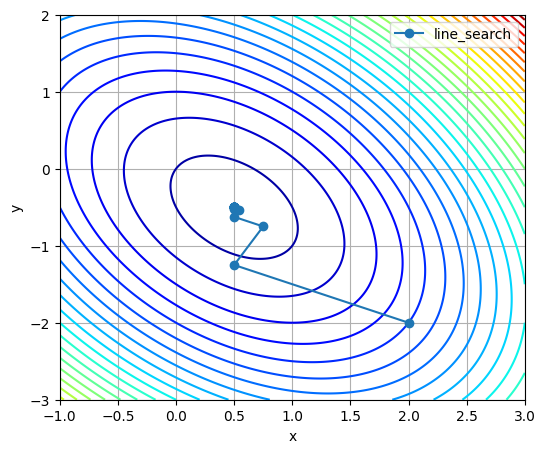
\includegraphics[width=\textwidth]{images/task2/plot_levels_2_2_line_search.png}
        \caption{Линии уровня, line\_search.}
    \end{minipage}\hfill
    \begin{minipage}{0.49\textwidth}
        \centering 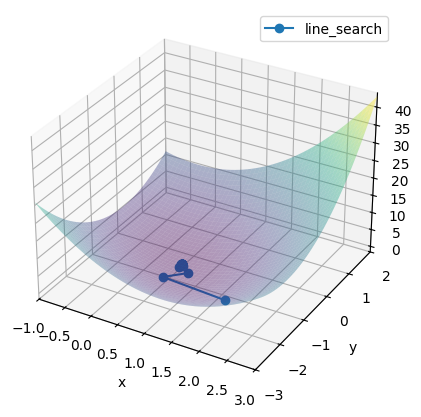
\includegraphics[width=0.84\textwidth]{images/task2/plot_3d_2_2_line_search.png}
        \caption{3D-график, line\_searc.}
    \end{minipage} 
\end{figure}
\begin{figure}[H]
    \begin{minipage}{0.49\textwidth}
        \centering 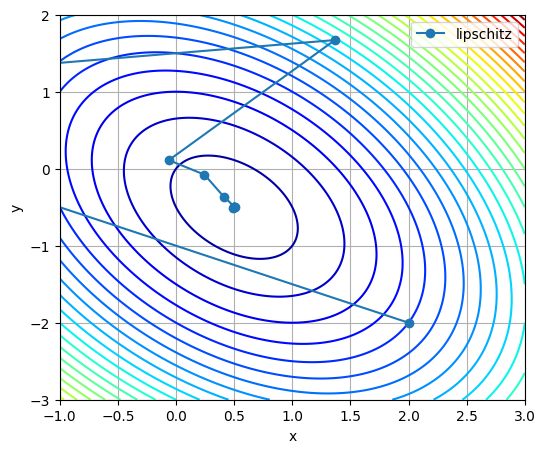
\includegraphics[width=\textwidth]{images/task2/plot_levels_2_2_lipschitz.png}
        \caption{Линии уровня, lipschitz.}
    \end{minipage}\hfill
    \begin{minipage}{0.49\textwidth}
        \centering 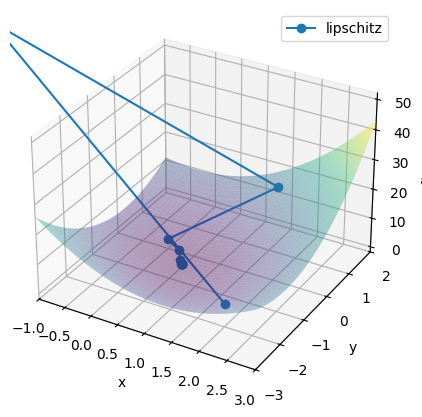
\includegraphics[width=0.84\textwidth]{images/task2/plot_3d_2_2_lipschitz.png}
        \caption{3D-график, lipschitz.}
    \end{minipage}
\end{figure}
\begin{figure}[H]
    \begin{minipage}{0.49\textwidth}
        \centering 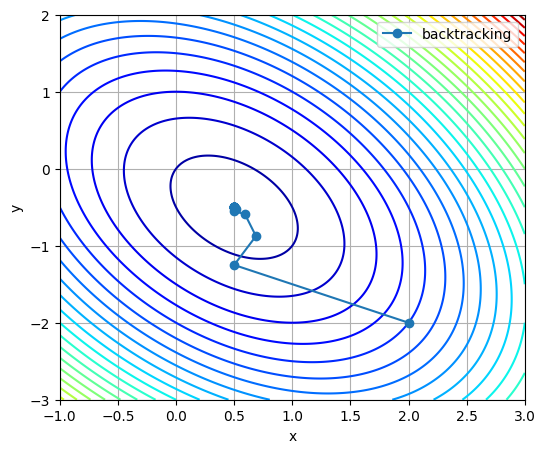
\includegraphics[width=\textwidth]{images/task2/plot_levels_2_2_backtracking.png}
        \caption{Линии уровня, backtracking.}
    \end{minipage}\hfill
    \begin{minipage}{0.49\textwidth}
        \centering 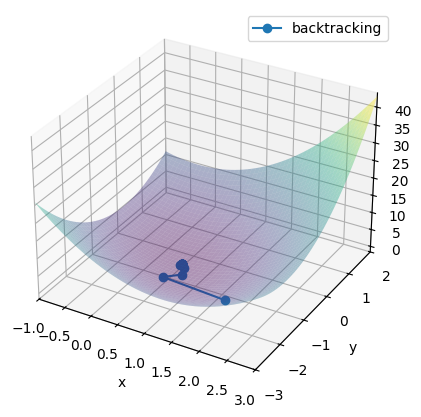
\includegraphics[width=0.84\textwidth]{images/task2/plot_3d_2_2_backtracking.png}
        \caption{3D-график, backtracking.}
    \end{minipage}
\end{figure}
\noindent
Видно, что:
\begin{itemize}
    \item constant идёт плавной дугой к минимуму, 
    \item lipschitz может «выстрелить» вверх, если локальная оценка $L_k$ мала.
    \item line\_search и backtracking делают более прямолинейные шаги,
\end{itemize}

Для наглядности построим график логарифмической ошибки $\|x_k - x^*\|$ от номера итерации для всех четырёх стратегий (constant, line\_search, lipschitz, backtracking).
\begin{figure}[H]
    \centering
    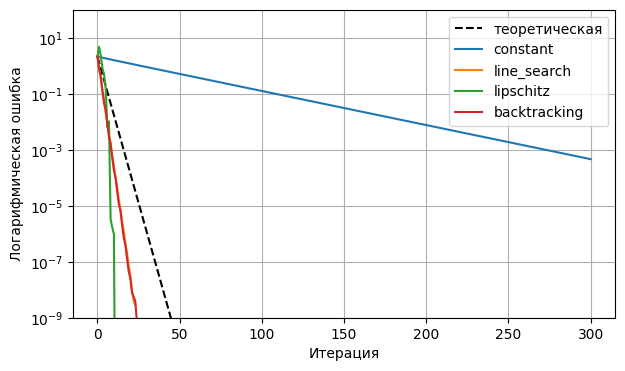
\includegraphics[width=0.6\textwidth]{images/task2/convergence_x_error_all_strategies.png}
    \caption{Сходимость для квадратичной задачи, все стратегии.}
\end{figure}
\noindent
Видно, что:
\begin{itemize}
    \item constant --- метод убывает примерно линейно, причём медленнее, чем теоретическая кривая $(1-\mu/L)^k$, если шаг не оптимален;
    \item line\_search и lipschitz показывают более резкий спад ошибки на первых шагах;
    \item backtracking (Армихо) часто выходит на минимальную ошибку быстрее всех.
\end{itemize}
\noindent
Теперь рассмотрим функцию Розенброка
$ f(x,y) \;=\; (1 - x)^2 \;+\; 100\,\bigl(y - x^2\bigr)^2,$
которая является классическим примером <<неудобной>> функции с узкой <<долиной>> вдоль параболы $y=x^2$. Мы вновь используем метод градиентного спуска в четырёх вариантах: constant, line\_search, lipschitz, backtracking, и сравниваем траектории.

Далее приведены 2D-графики для каждой стратегии и та же функция в виде 3D-поверхности $z=f(x,y)$ и траектории $\{x_k\}$.

\begin{figure}[H]
    \centering
    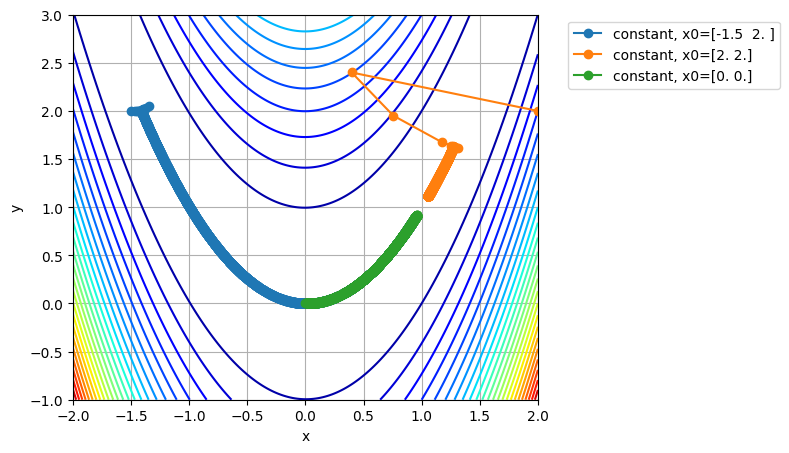
\includegraphics[width=0.8\textwidth]{images/task2/plot_levels_2_3_constant.png}
    \caption{Линии уровня, constant.}
\end{figure}
\begin{figure}[H]
    \centering
    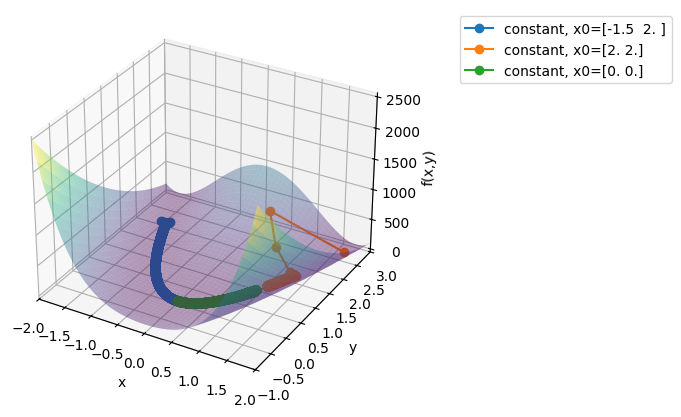
\includegraphics[width=0.8\textwidth]{images/task2/plot_3d_2_3_constant.png}
    \caption{3D-график, constant.}
\end{figure}

\begin{figure}[H]
    \centering
    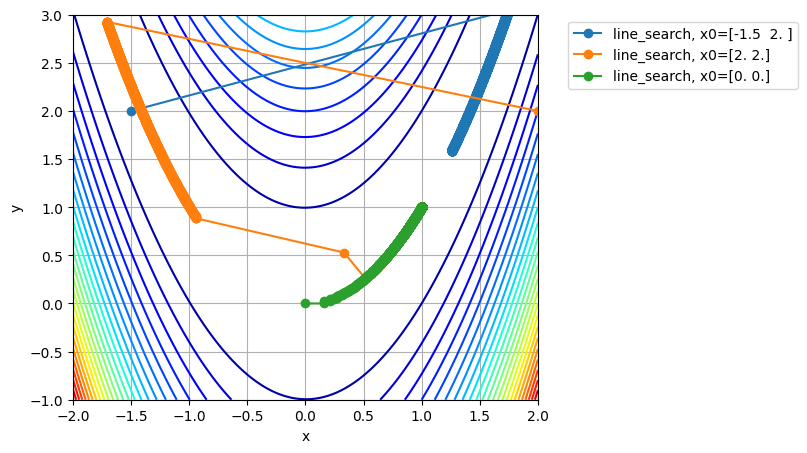
\includegraphics[width=0.8\textwidth]{images/task2/plot_levels_2_3_line_search.png}
    \caption{Линии уровня, line\_search.}
\end{figure}
\begin{figure}[H]
    \centering
    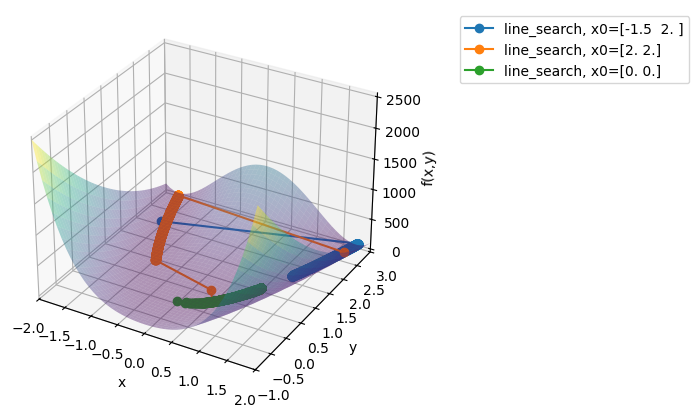
\includegraphics[width=0.8\textwidth]{images/task2/plot_3d_2_3_line_search.png}
    \caption{3D-график, line\_search.}
\end{figure}

\begin{figure}[H]
    \centering
    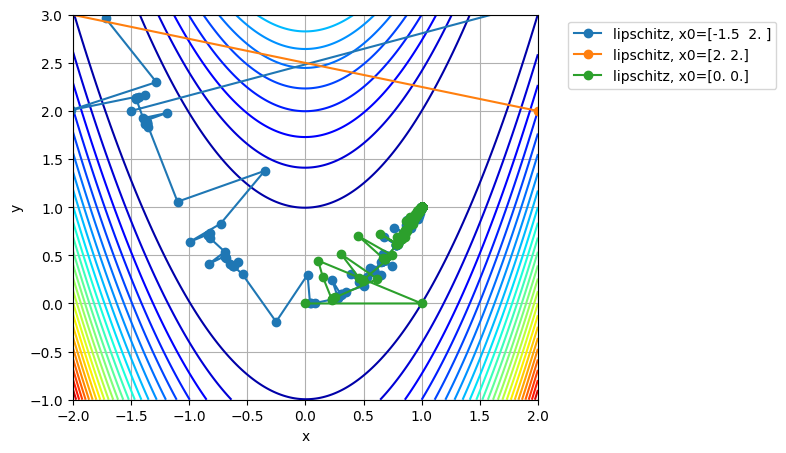
\includegraphics[width=0.8\textwidth]{images/task2/plot_levels_2_3_lipschitz.png}
    \caption{Линии уровня, lipschitz.}
\end{figure}
\begin{figure}[H]
    \centering
    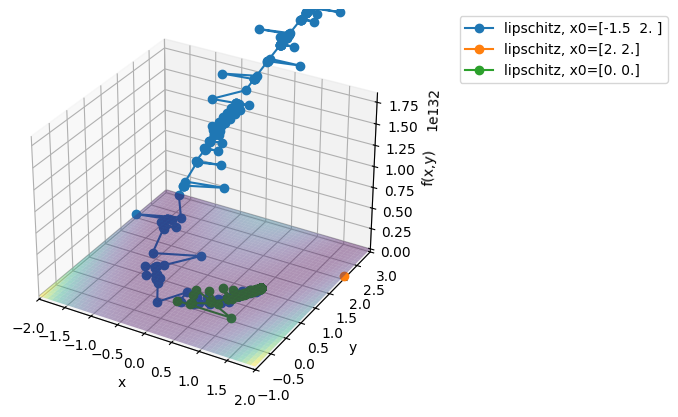
\includegraphics[width=0.8\textwidth]{images/task2/plot_3d_2_3_lipschitz.png}
    \caption{3D-график, lipschitz.}
\end{figure}

\begin{figure}[H]
    \centering
    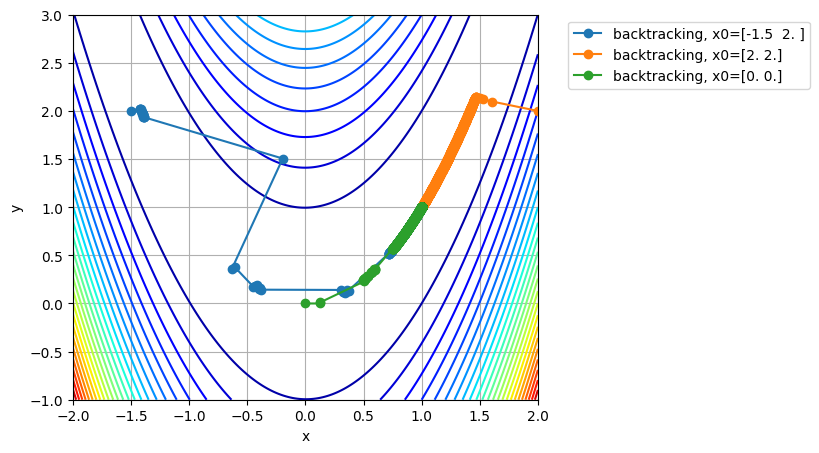
\includegraphics[width=0.8\textwidth]{images/task2/plot_levels_2_3_backtracking.png}
    \caption{Линии уровня, backtracking.}
\end{figure}
\begin{figure}[H]
    \centering
    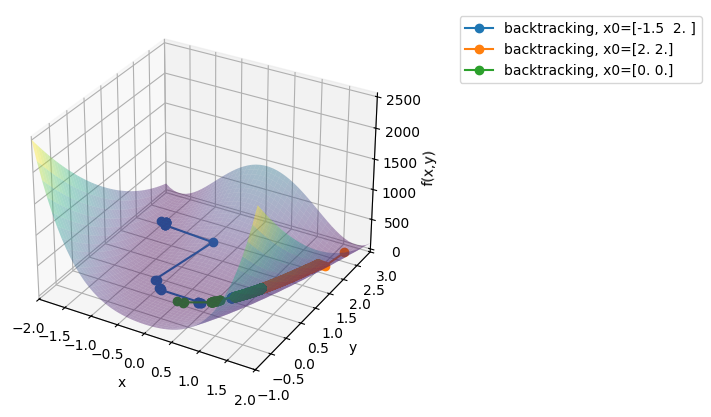
\includegraphics[width=0.8\textwidth]{images/task2/plot_3d_2_3_backtracking.png}
    \caption{3D-график, backtracking.}
\end{figure}

Как видно из 2D-графиков, функция Розенброка имеет минимум в $(1,1)$, но <<долина>> довольно узкая и <<крутая>>. 
\begin{itemize}
    \item constant рисует плавную (иногда изогнутую) траекторию, поскольку шаг зафиксирован и не учитывает геометрию долины.
    \item line\_search делает более прямолинейные отрезки, подбирая шаг через одномерную оптимизацию.
    \item lipschitz может <<выстрелить>> наверх, если локальная оценка $L_k$ занижена, что приводит к очень большим значениям $f$ на какой-то итерации.
    \item backtracking даёт <<осторожные>> шаги, сохраняя условие Армихо $f(x_{k+1}) \le f(x_k) - c\,\alpha_k \|\nabla f(x_k)\|^2$, и в итоге часто даёт самую ровную сходимость.
\end{itemize}

Чтобы наглядно сравнить скорость сходимости различных стратегий градиентного спуска на функции Розенброка, построим графики зависимости $\|x_k - (1,1)\|$ от номера итерации $k$ при трёх разных начальных приближениях.
\begin{figure}[H]
    \centering
    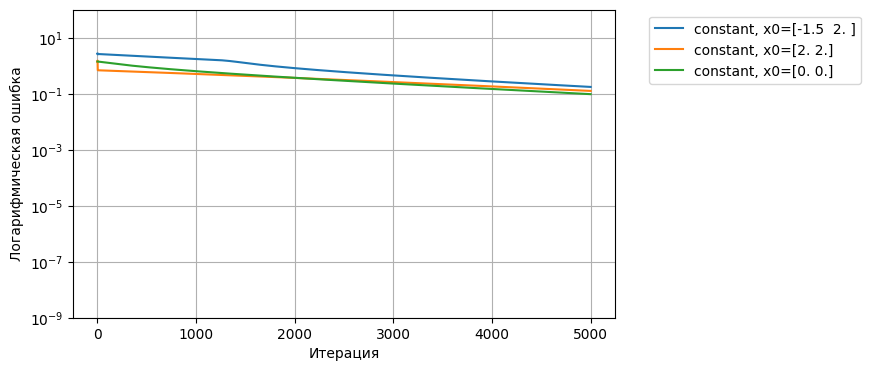
\includegraphics[width=0.8\textwidth]{images/task2/convergence_x_error_2_3_constant.png}
    \caption{Логарифмическая ошибка по $x$ для constant, несколько $x_0$.}
\end{figure}
\begin{figure}[H]
    \centering
    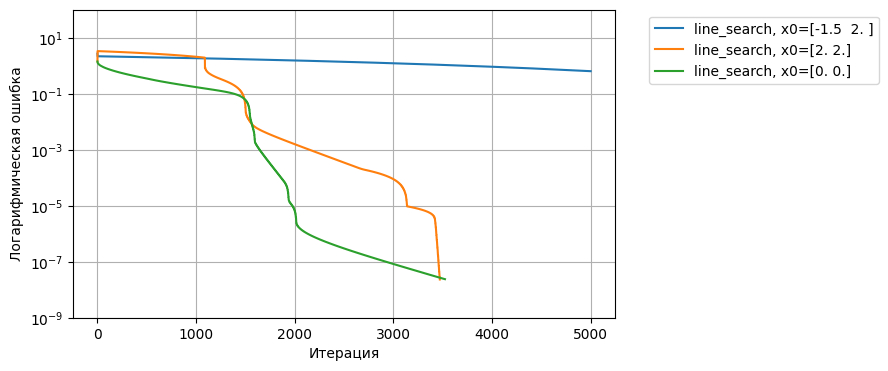
\includegraphics[width=0.8\textwidth]{images/task2/convergence_x_error_2_3_line_search.png}
    \caption{Логарифмическая ошибка по $x$ для line\_search, несколько $x_0$.}
\end{figure}
\begin{figure}[H]
    \centering
    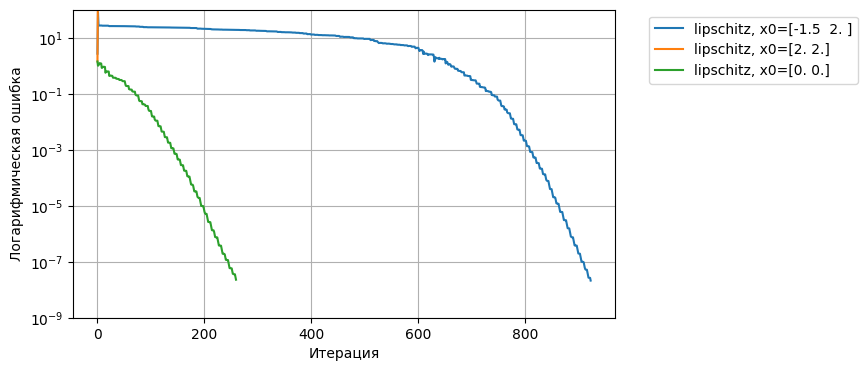
\includegraphics[width=0.8\textwidth]{images/task2/convergence_x_error_2_3_lipschitz.png}
    \caption{Логарифмическая ошибка по $x$ для lipschitz, несколько $x_0$.}
\end{figure}
\begin{figure}[H]
    \centering
    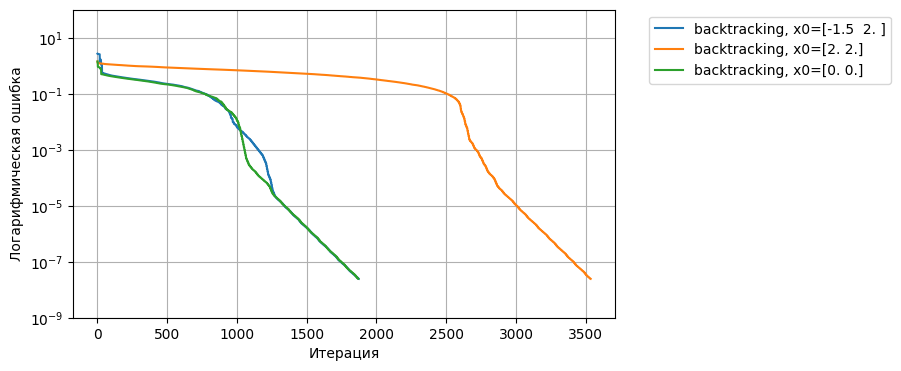
\includegraphics[width=0.8\textwidth]{images/task2/convergence_x_error_2_3_backtracking.png}
    \caption{Логарифмическая ошибка по $x$ для backtracking, несколько $x_0$.}
\end{figure}
\noindent
На всех четырёх графиках видно, что:
\begin{itemize}
    \item Backtracking показывает довольно <<плавную>> убывание ошибки, однако при стартовой точке $(2,2)$ метод расходует гораздо больше итераций (около 3000--3500), прежде чем достичь ошибки порядка $10^{-8}$. Для ближних стартов $(0,0)$ или $(-1.5,2)$ кривая убывает быстрее.
    \item Constant сходится равномерно, но достаточно медленно (кривая примерно линейна по оси итераций); за 5000 итераций ошибка падает к $10^{-8}$. При разных $x_0$ кривая смещается, но форма остаётся похожей.
    \item Line\_search даёт <<ступенчатое>> поведение: например, при $(2,2)$ ошибка долго <<застывает>> на уровне $10^{-1}$, а затем быстро <<проваливается>> к $10^{-7}$. При $(0,0)$ сходится ещё быстрее.
    \item Lipschitz при удачном старте (зелёная кривая) даёт стремительное падение ошибки всего за 200--300 итераций; при неудачном (синяя кривая) метод сначала может <<улетать>> на огромные значения, но в итоге всё же <<возвращается>> и убывает до $10^{-9}$.
\end{itemize}

\subsection{Вывод}
\begin{itemize}
    \item Для квадратичной функции $f(x)=x^\mathsf{T}Ax + b^\mathsf{T}x$ все четыре стратегии (constant, line\_search, lipschitz, backtracking) гарантированно находят минимум, причём line search и backtracking часто выходят на заданную точность заметно быстрее, чем constant. Lipschitz тоже может быть эффективен, если локальные оценки $L_k$ не <<врут>> слишком сильно.
    \item Для функции Розенброка также все методы в итоге сходятся к глобальному минимуму $(1,1)$, но:
    \begin{itemize}
        \item line\_search и backtracking в большинстве случаев дают стабильную сходимость без резких скачков;
        \item lipschitz может <<выпрыгивать>> на большие значения, если $L_k$ оказывается заниженным, особенно при далёком $x_0$;
        \item constant требует подбора $\alpha$, иначе метод <<ползёт>> очень долго или начинает <<болтаться>>.
    \end{itemize}
    \item В обоих примерах backtracking часто даёт наиболее <<гладкую>> кривую убывания ошибки, хотя иногда требует дополнительных итераций, если стартовая точка далека.
\end{itemize}

Таким образом, все четыре стратегии работоспособны, но скорость и стабильность зависят от свойств задачи (выпуклость, глобальная/локальная липшицевость) и от начального приближения. 
\section{Построение траектории}
\subsection{Постановка задачи и её разрешение}
В данном задании мы попробуем применить метод градиентного спуска для решения практической задачи. Нам необходимо, в лице робота, пройти из точки A в B, учитывая препятствия.
\\
\\
Для построения нашей "полосы препятствий" мы восползуемся потенциальной функцией вида:
$$F(x,y) = a((x-x_b)^2+(y-y_b)^2)+\sum_1^n b_iexp({-\frac{{(x-x_{p_i})}^2}{2\sigma_{x_i}}-\frac{{(y-y_{p_i})}^2}{2\sigma_{y_i}}})$$
\\
Данная функция, по своей сути, строит квадратичную функцию с точкой минимума в $(x_b,y_b)$ и добавляет гауссовы колокола вокруг. В общем то, из-за того, что эти колокола вне своих "радиусов" очень быстро приближаются к нулю, прибавления таких функций глобально не повлияет на расположение минимума.
\\
Раcсмотрим наши параметры для этой функции:
\begin{itemize}
\item $(x_b,y_b) = (6,4)$
\item $a = 0.1$ -коэффициент квадратичной функции. Взяли его таким маленьким, потому что при больших значениях он очень быстро перекрывает колокол
\item Высота колоколов, за которые отвечают коэффициенты $b_i$ варьируется в интервале от 20 до 60
\item "Радиусы" колоколов все равны 0.8.
\item И, конечно, точки - центры колоколов:(3,2),(-3,-2),(3,8),(3,-2)
\end{itemize}
Для данной функции воспользуемся довольно простым методом - будем подбирать коэффициент перед градиентом с помощью оптимизации функции одной переменной. \\[0.5em]
Посмотрим на то, какой получился траектория(для начальной точки(-6,-6)):
\begin{figure}[H]
    \centering
    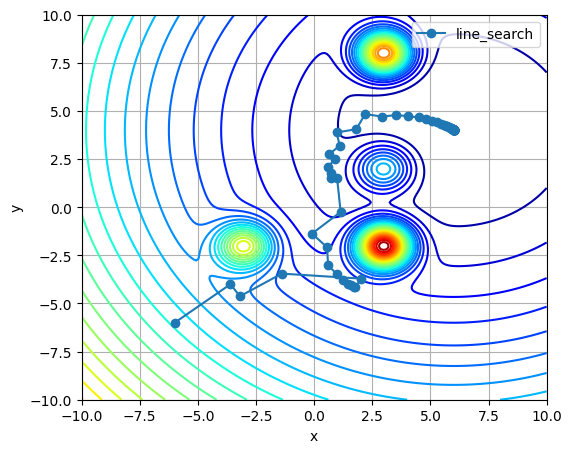
\includegraphics[width=0.8\textwidth]{images/task3/plot_levels_3_potential.png}
    \caption{2D-график, line\_search.}

    \centering
    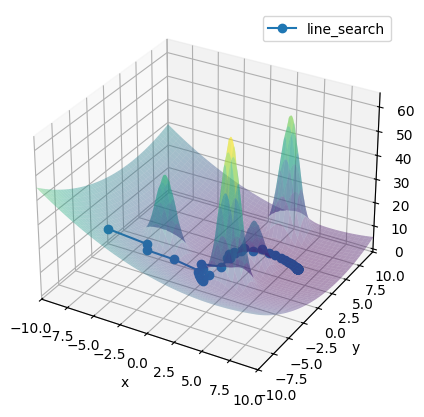
\includegraphics[width=0.8\textwidth]{images/task3/plot_3d_3_potential.png}
    \caption{3D-график, line\_search.}
\end{figure}
\noindent
Как можно наблюдать - метод справился! Полученная точка $\approx (6.01,4.01)$. Небольшая ошибка возникла по двум причинам: ошибка численного вычисления градиента и очень маленькое значение градиента вблизи точки минимума. А ведь критерий для остановки нашего алгоритма завязан на модуле градиента\dots В общем, причина ошибки достаточно понятна.\\[0.5em]
Давайте также обратим внимание на траекторию - она получилась достаточно ровной, без сильных перелётов. Возможно, настоящий робот даже сможет по ней проехать. \\[0.5em]
Стоит сделать небольшое признание. Хотя для этой конкретной конфигурации наш метод линейного поиска и справился, но стоит понимать, что, к примеру, если даже немного сдвинуть колокол в точке (3,8) ближе к центру координат, то наш метод застрянет между двух колоколов и не спустится в точку минимума. \\[0.5em]
Немного про полученную траекторию. В данном случае можно наблюдать, что в дали от точки минимума(когда градиент значительный) наш метод довольно хорошо проскакивает к условно минимальным точкам, может сделать достаточно значительнео перемешение за 2-3 шага. Но вот приближившись к минимуму происходит быстрое уменьшение шага. Также достаточно интересным является то, что наш метод в какой то момент пытается практически упереться в вершину холма. Такое поведения могло бы оказаться фатальным для сходимости метода, тем не менее он довольно хорошо вышел из ситуации.
\subsection{Вывод}
В данном разделе нам удалось применить полученные знания и методы для решения практической задачи. Как оказалось, метод градиентного спуска можно применять довольно креативно - не только искать минимумы разлиных функций, но и использовать данные об траектории метода, чтобы самим строить траекторию робота. Также выяснилось, что для решения этой задачи может подойти достаточна простая стратегия для выбора коэффициента в градиентном методе, хотя и условия для использования должны быть в каком-то смыле "стерильными".
\end{document}
